% The mini rig seen from the front, traced from a photo of a finished rig:
% the acrylic panel with its engraved bike, and the hardware the control
% system uses. The breadboard and Arduino sit on top and are left out.
\documentclass[border=2pt]{standalone}
\usepackage[svgnames]{xcolor}
\usepackage{tikz}
\usetikzlibrary{calc}
\definecolor{panel}{RGB}{176,138,214}
\definecolor{crankarm}{RGB}{255,120,30}
\definecolor{servoblue}{RGB}{40,70,200}

\begin{document}
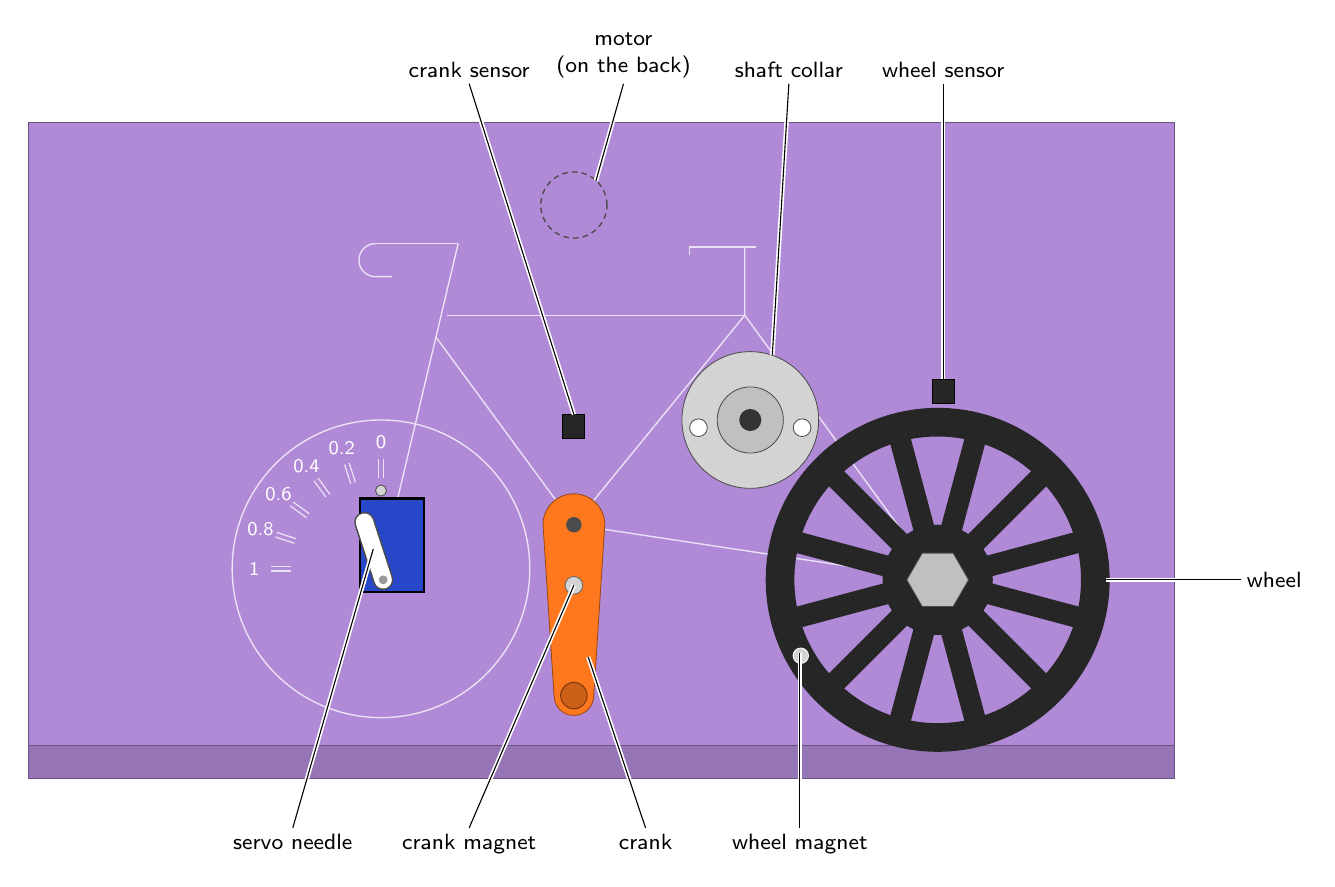
\begin{tikzpicture}[
    x=1.4cm, y=1.4cm,
    engraving/.style={draw=white!75!panel, line width=.5pt},
    label/.style={font=\sffamily\footnotesize, inner sep=2pt},
    leader/.style={draw=black, line width=.4pt,
        preaction={draw=white, line width=1.6pt}},
    sensor/.style={fill=black!85, draw=black},
]
    %% the panel and its foot
    \filldraw[fill=panel, draw=panel!60!black, line width=.4pt]
        (0, .3) rectangle (10.4, 5.95);
    \filldraw[fill=panel!85!black, draw=panel!60!black, line width=.4pt]
        (0, 0) rectangle (10.4, .3);

    %% the bike engraved on the panel
    \draw[engraving] (3.2, 1.9) circle (1.35);
    \draw[engraving] (3.9, 4.85) -- (3.2, 1.9);                % fork
    \draw[engraving] (3.15, 4.85) -- (3.9, 4.85);              % handlebar
    \draw[engraving] (3.15, 4.85) arc[start angle=90, end angle=270,
        radius=.15] -- (3.3, 4.55);
    \draw[engraving] (3.8, 4.2) -- (6.5, 4.2);                 % top tube
    \draw[engraving] (3.7, 4.0) -- (4.95, 2.3);                % down tube
    \draw[engraving] (6.5, 4.82) -- (6.5, 4.2) -- (4.95, 2.3); % seat tube
    \draw[engraving] (6.5, 4.2) -- (8.25, 1.8);                % seat stay
    \draw[engraving] (4.95, 2.3) -- (8.25, 1.8);               % chain stay
    \draw[engraving] (6.0, 4.75) -- (6.0, 4.82) -- (6.6, 4.82); % saddle

    %% the motor demand scale, engraved as slots around the front wheel's
    %% centre: 0 straight up, 1 pointing forwards
    \foreach \v/\t in {0/0, .2/0.2, .4/0.4, .6/0.6, .8/0.8, 1/1} {
        \draw[engraving, double=panel, double distance=1.2pt]
            (3.2, 1.9) ++(90+90*\v:.82) -- ++(90+90*\v:.18);
        \node[font=\sffamily\scriptsize, text=white, inner sep=0pt]
            at ($(3.2, 1.9) + (90+90*\v:1.15)$) {\t};
    }

    %% the servo in its cut-out, with the horn as the needle
    \filldraw[fill=servoblue, draw=black, line width=1pt]
        (3.01, 1.69) rectangle (3.59, 2.54);
    \filldraw[fill=LightGray, draw=black!70, line width=.3pt] (3.2, 2.61)
        circle (.05);
    \draw[line width=.26cm, draw=black!70, line cap=round]
        (3.22, 1.8) -- ++(108:.55);
    \draw[line width=.22cm, draw=white, line cap=round]
        (3.22, 1.8) -- ++(108:.55);
    \fill[black!40] (3.22, 1.8) circle (.04);

    %% the crank, hanging down, with its magnet and its sensor above
    \filldraw[fill=crankarm, draw=crankarm!60!black, line width=.3pt]
        (4.67, 2.3) arc[start angle=180, end angle=0, radius=.28]
        -- (5.13, .75) arc[start angle=0, end angle=-180, radius=.18]
        -- cycle;
    \filldraw[fill=crankarm!80!black, draw=crankarm!50!black] (4.95, .75)
        circle (.12);
    \fill[black!70] (4.95, 2.3) circle (.07);
    \filldraw[fill=LightGray, draw=black!60, line width=.3pt] (4.95, 1.75)
        circle (.08);
    \fill[sensor] (4.85, 3.08) rectangle (5.05, 3.3);

    %% the motor, hidden on the back of the panel, so drawn dashed
    \draw[black!70, line width=.5pt, dash pattern=on 2pt off 1.5pt]
        (4.95, 5.2) circle (.3);

    %% the shaft collar, on the shaft that carries the gear on the back
    \filldraw[fill=LightGray, draw=black!70, line width=.3pt] (6.55, 3.25)
        circle (.62);
    \filldraw[fill=Silver, draw=black!70, line width=.3pt] (6.55, 3.25)
        circle (.3);
    \fill[black!80] (6.55, 3.25) circle (.1);
    \foreach \dx in {-.47, .47}
        \filldraw[fill=white, draw=black!70, line width=.3pt]
            (6.55+\dx, 3.18) circle (.08);

    %% the wheel, with its magnet and its sensor above
    \begin{scope}[shift={(8.25, 1.8)}]
        % rim, hub and twelve straight spokes
        \fill[black!85, even odd rule] (0, 0) circle (1.56) circle (1.3);
        \fill[black!85] (0, 0) circle (.5);
        \foreach \a in {15, 45, ..., 345}
            \draw[black!85, line width=.27cm] (\a:.45) -- (\a:1.35);
        % the axle bolt
        \filldraw[fill=Silver, draw=black!70, line width=.3pt]
            (0:.28) \foreach \a in {60, 120, ..., 300} {-- (\a:.28)} -- cycle;
        \filldraw[fill=LightGray, draw=white, line width=.3pt] (209:1.42)
            circle (.07);
    \end{scope}
    \fill[sensor] (8.2, 3.4) rectangle (8.4, 3.62);

    %% labels
    \draw[leader] (3.13, 2.08) -- (2.4, -.45) node[label, anchor=north]
        {servo needle};
    \draw[leader] (4.95, 3.3) -- (4.0, 6.3) node[label, anchor=south]
        {crank sensor};
    \draw[leader] (5.15, 5.42) -- (5.4, 6.3) node[label, anchor=south,
        align=center] {motor\\(on the back)};
    \draw[leader] (6.75, 3.84) -- (6.9, 6.3) node[label, anchor=south]
        {shaft collar};
    \draw[leader] (8.3, 3.62) -- (8.3, 6.3) node[label, anchor=south]
        {wheel sensor};
    \draw[leader] (4.95, 1.75) -- (4.0, -.45) node[label, anchor=north]
        {crank magnet};
    \draw[leader] (5.08, 1.1) -- (5.6, -.45) node[label, anchor=north]
        {crank};
    \draw[leader] (7.0, 1.14) -- (7.0, -.45) node[label, anchor=north]
        {wheel magnet};
    \draw[leader] (9.78, 1.8) -- (11, 1.8) node[label, anchor=west]
        {wheel};
\end{tikzpicture}
\end{document}
